\documentclass{article}

\usepackage[main, final]{neurips_2026}

\makeatletter
\renewcommand{\@notice}{}
\makeatother

\usepackage[utf8]{inputenc}
\usepackage[T1]{fontenc}
\usepackage{hyperref}
\usepackage{url}
\usepackage{booktabs}
\usepackage{multirow}
\usepackage{amsfonts}
\usepackage{amsmath}
\usepackage{amssymb}
\usepackage{nicefrac}
\usepackage{microtype}
\usepackage{xcolor}
\usepackage{graphicx}
\usepackage{subcaption}
\usepackage{placeins}
\usepackage{cleveref}

\title{Inductive Biases for Forecasting}

\author{%
  Abdul Hafeez \\
  \texttt{25280098@lums.edu.pk}
}

\renewcommand{\topfraction}{0.85}
\renewcommand{\bottomfraction}{0.6}
\renewcommand{\textfraction}{0.1}
\renewcommand{\floatpagefraction}{0.8}
\setcounter{totalnumber}{5}

\begin{document}

\maketitle

All code and reproducible experiments are hosted at \url{https://github.com/hafeez381/autoformer-forecasting}.

\section{Forecasting Across Heterogeneous Sensors}
\label{sec:t1}
\label{subsec:t1-setup}

We forecast the next $H = 48$ vibration readings of one station at a production line from its last $L = 96$, where each reading is the sum of a slow drift, a cycle whose period $P$ depends on the current product, and noise. Ridge regression, i.e. least squares with a small weight penalty, fits one matrix $\hat W \in \mathbb{R}^{L \times H}$ that is applied to every context, while self-attention learns projections $W_Q$, $W_K$ and $W_V$ and computes its attention weights $\mathrm{softmax}(QK^\top/\sqrt{d_h})$ from each context, with $Q = XW_Q$, $K = XW_K$ and head width $d_h$. We test how much this context dependence helps, and whether two inductive biases, moving-average decomposition for the slow drift and delay mixing for repetition, help more than added flexibility. All results come from one full-preset run with seed 0. We report validation RMSE in m/s$^2$ on the established Stations 1--3 and the held-out Station 4.

\subsection{Context-Dependent Forecasting}
\label{subsec:t1-context}

\paragraph{Response 1A.}

Before Output 1.1 ran, we predicted period-routed ridge, then Raw Attention, shared ridge and sensor-specific ridge on the established stations, and the same order without sensor-specific ridge on Station 4, because period routing keeps windows of different periods apart, Raw Attention has more capacity than one shared $\hat W$ but cannot handle the slow drift, and sensor-specific ridge fits each $\hat W$ on only a third of the training windows. Both orderings held (Table~\ref{tab:t1-products}). Period routing had the lowest validation RMSE on both populations (0.166 on the established stations, 0.173 on Station 4), $4.6\times$ below shared ridge (0.767). Sensor-specific ridge tied shared ridge (0.768 vs.\ 0.767), as station identity says nothing about the period. Raw Attention beat both fixed ridges without period information (0.424) but had $2.6\times$ the RMSE of period routing, and its RMSE rose the most on Station 4 (0.424 to 0.617, $+46\%$), likely from fitting station-specific patterns.

On the established stations, shared ridge did best on Product C (0.621) and worst on B (0.854), while period routing did best on C (0.152) and worst on A (0.181). Period routing assumes one $\hat W$ per period band, and a fixed-width band is coarse for short periods, so A windows in one band differ more in phase. Shared ridge assumes one $\hat W$ for every period, which costs least on C, whose long cycle changes less over 48 steps. We keep both orderings but expect a much larger gap between period routing and Raw Attention.

\begin{table}[!htbp]
  \centering
  \caption{Validation RMSE (m/s$^2$) overall and per product of the Part 1 forecasters (Output 1.1) and of Raw Attention with the width-41 decomposition (Output 2.3).}
  \label{tab:t1-products}
  \small
  \resizebox{\linewidth}{!}{\begin{tabular}{l cccc cccc}
\toprule
& \multicolumn{4}{c}{\textbf{Established (1--3)}} & \multicolumn{4}{c}{\textbf{Station 4}} \\
\cmidrule(lr){2-5}\cmidrule(lr){6-9}
\textbf{Model} & All & A & B & C & All & A & B & C \\
\midrule
Shared ridge & $0.767$ & $0.805$ & $0.854$ & $0.621$ & $0.876$ & $0.909$ & $0.982$ & $0.713$ \\
Sensor-specific ridge & $0.768$ & $0.804$ & $0.852$ & $0.630$ & -- & -- & -- & -- \\
Period-routed ridge & $0.166$ & $0.181$ & $0.164$ & $0.152$ & $0.173$ & $0.184$ & $0.182$ & $0.150$ \\
Raw Attention & $0.424$ & $0.387$ & $0.476$ & $0.405$ & $0.617$ & $0.649$ & $0.578$ & $0.621$ \\
\midrule
Attention + decomposition & $0.296$ & $0.267$ & $0.336$ & $0.281$ & $0.444$ & $0.375$ & $0.496$ & $0.453$ \\
\bottomrule
\end{tabular}
}
\end{table}

\paragraph{Response 1B.}

On the Product A window of Output 1.2 (Figure~\ref{fig:t1-forecasts}), shared and sensor-specific ridge forecast peaks that are too small and too early (RMSE 0.779 and 0.787 vs.\ 0.232 for period routing, Table~\ref{tab:t1-windows}). One $\hat W$ must fit contexts that need different phase shifts, so the least-squares solution averages them into a smaller, out-of-phase forecast.

Raw Attention's $W_Q$, $W_K$ and $W_V$ are fixed after training, but $QK^\top$ is recomputed for each window, so each context gets its own attention matrix and mixes $V$ differently. The Product A and Product C attention matrices differed by 0.011 on average and by up to 0.437 (Table~\ref{tab:t1-attention}), whereas ridge regression applies the same $\hat W$ to both.

\begin{figure}[!htbp]
  \centering
  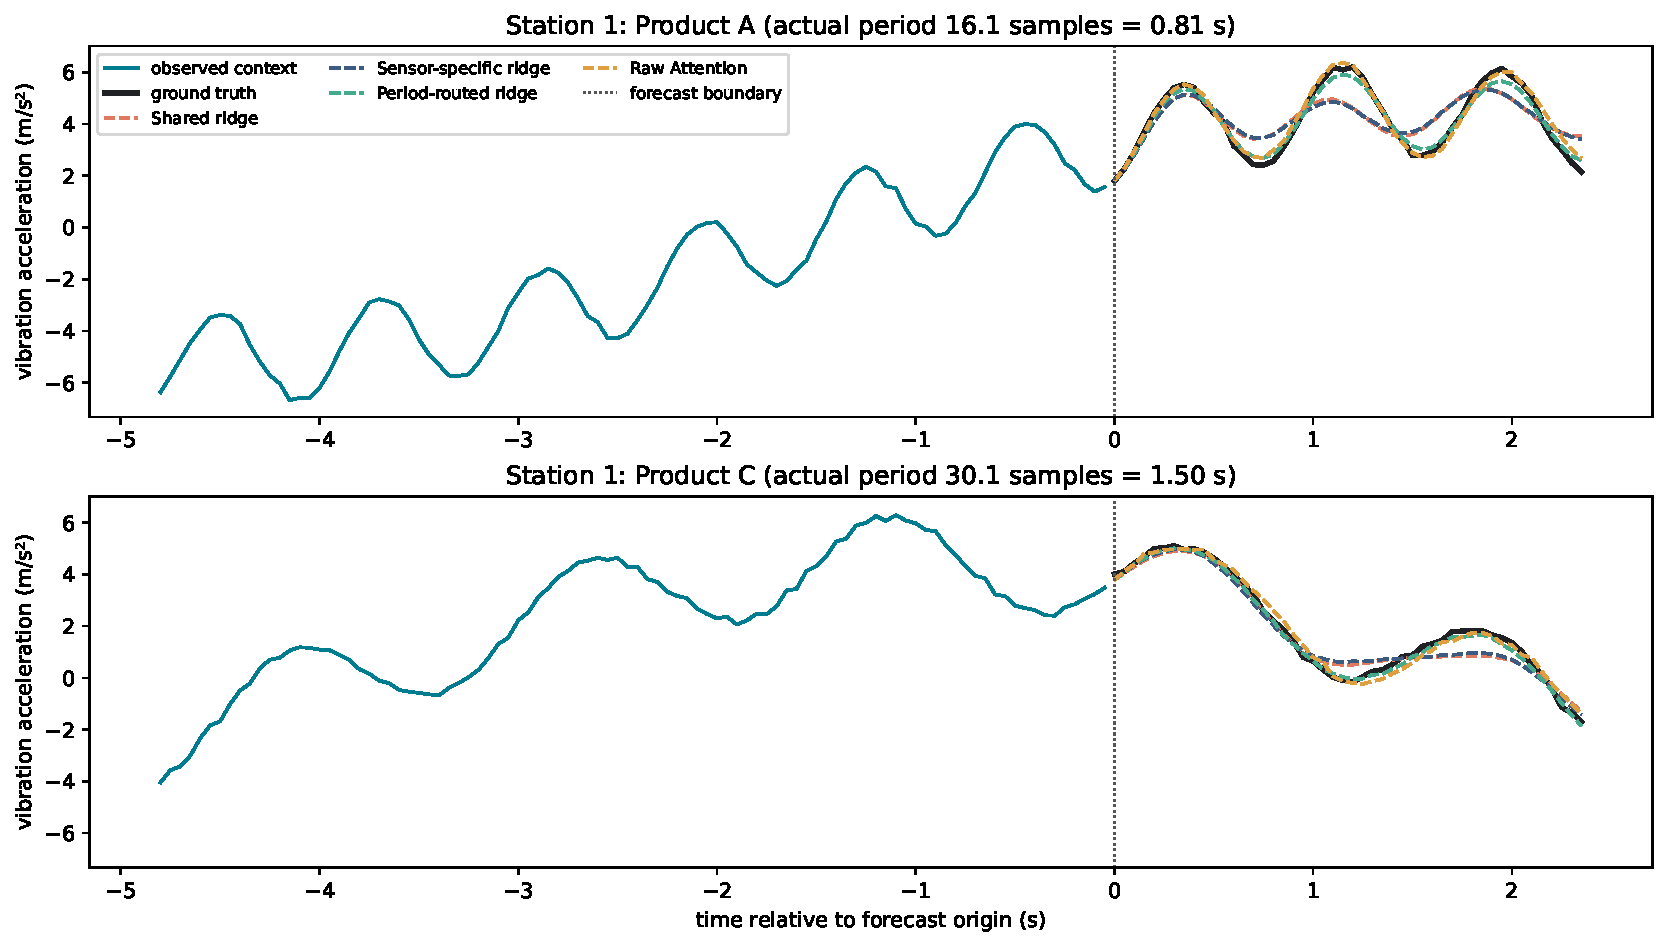
\includegraphics[width=0.8\linewidth]{figures/t1_out1-2.pdf}
  \caption{Validation forecasts on two Station 1 windows, Product A with period 16.1 (top) and Product C with period 30.1 (bottom), in m/s$^2$ (Output 1.2).}
  \label{fig:t1-forecasts}
\end{figure}

\begin{table}[!htbp]
  \centering
  \caption{Validation RMSE of each Part 1 forecaster on the two windows of Figure~\ref{fig:t1-forecasts} (Output 1.2).}
  \label{tab:t1-windows}
  \small
  \begin{tabular}{rlrlr}
\toprule
station & product & actual period (samples) & model & window RMSE (m/s²) \\
\midrule
1 & Product A & 16.135 & Shared ridge & 0.779 \\
1 & Product A & 16.135 & Sensor-specific ridge & 0.787 \\
1 & Product A & 16.135 & Period-routed ridge & 0.232 \\
1 & Product A & 16.135 & Raw Attention & 0.229 \\
1 & Product C & 30.093 & Shared ridge & 0.448 \\
1 & Product C & 30.093 & Sensor-specific ridge & 0.436 \\
1 & Product C & 30.093 & Period-routed ridge & 0.150 \\
1 & Product C & 30.093 & Raw Attention & 0.249 \\
\bottomrule
\end{tabular}

\end{table}

\begin{table}[!htbp]
  \centering
  \caption{Mean and maximum absolute difference between the head-averaged first-layer Raw Attention weights of the two windows of Figure~\ref{fig:t1-forecasts}, under the same $W_Q$, $W_K$, $W_V$ (Output 1.3).}
  \label{tab:t1-attention}
  \resizebox{\linewidth}{!}{\begin{tabular}{rlrrr}
\toprule
station & product & actual period (samples) & mean |Attention weight difference| & max |Attention weight difference| \\
\midrule
1 & Product A & 16.135 & unavailable & unavailable \\
1 & Product C & 30.093 & unavailable & unavailable \\
1 & Product A vs Product C (difference) & unavailable & 0.011 & 0.437 \\
\bottomrule
\end{tabular}
}
\end{table}

\subsection{Separating Slow Structure from Repetition}
\label{subsec:t1-decomp}

\paragraph{Response 2.}

A period-recovery check (oracle diagnostic) on training windows picked moving-average width $m = 41$. In Output 2.1, wider windows gave smoother trends (Figure~\ref{fig:t1-filter}, left) and larger remainders (Figure~\ref{fig:t1-filter}, middle), because less of the cycle went into the trend. The period score of the remainder peaked at the true period, while the score of the raw context was flat (Figure~\ref{fig:t1-filter}, right). Decomposition raised the fraction of training windows whose period was recovered within one sample from 0.687 for the raw context to 0.998 at width 41 (Table~\ref{tab:t1-recovery}). Adding it to Raw Attention lowered validation RMSE for every product on both populations, from 0.424 to 0.296 on the established stations and from 0.617 to 0.444 on Station 4 (Table~\ref{tab:t1-products}).

A moving average is a sensible bias here because the data is a slow drift plus a faster cycle, and a moving average keeps slow changes and smooths out fast ones. The period-recovery check is a useful way to pick its width because it tests what the split is for, recovering the cycle's period from the remainder, and it uses only training windows. This bias fails on a sudden jump in level, which the moving average spreads over $m$ samples, leaving a false bump in the remainder.

\begin{figure}[!htbp]
  \centering
  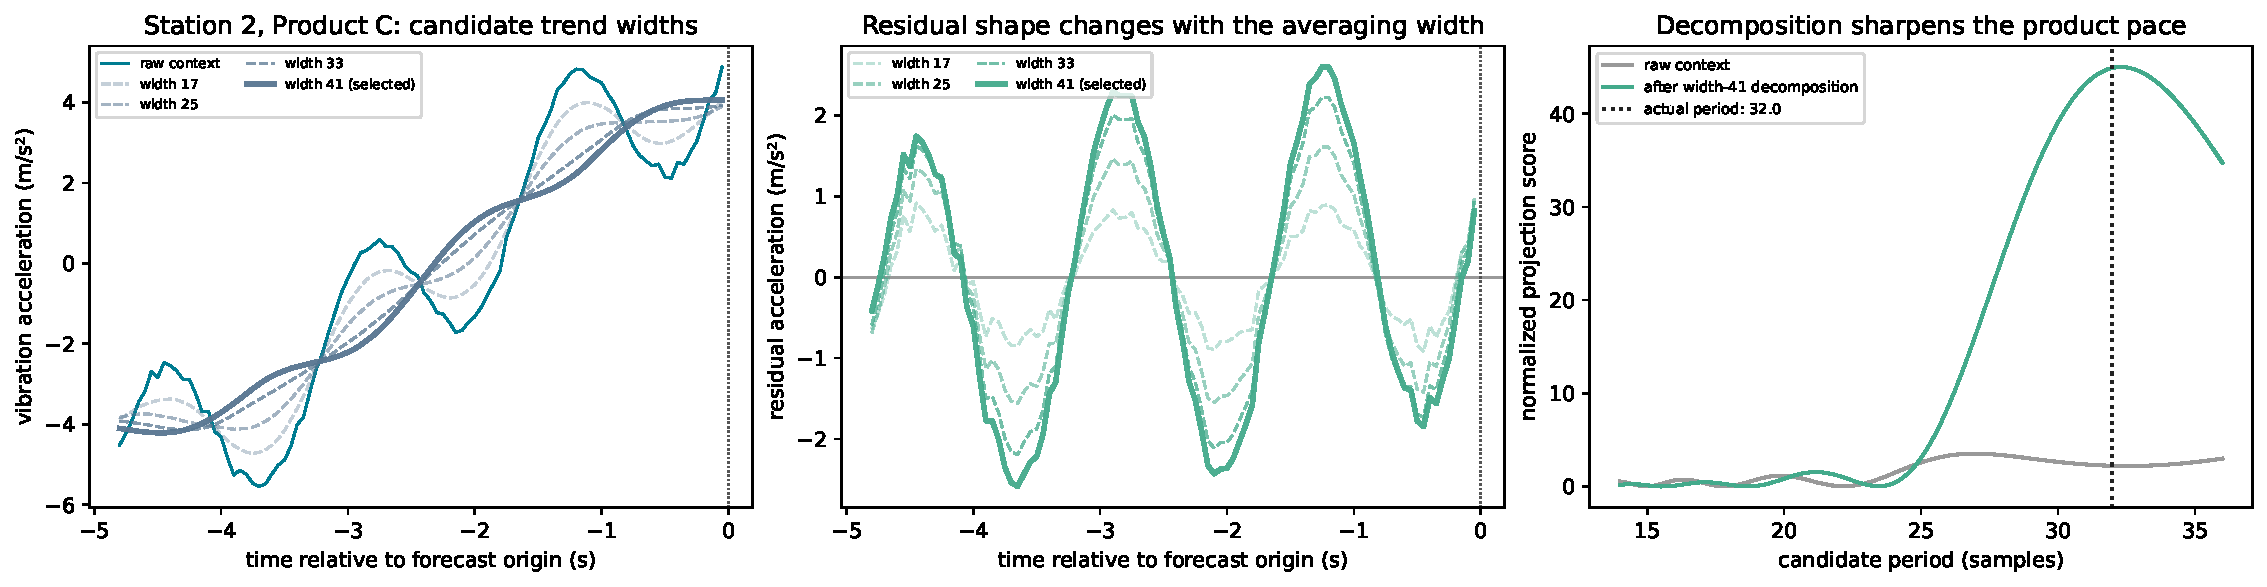
\includegraphics[width=\linewidth]{figures/t1_out2-1.pdf}
  \caption{Trends (left) and remainders (middle) of one Station 2 Product C validation context for widths 17 to 41, and the period score of the raw context and the width-41 remainder (right), with the true period of 32.0 dotted (Output 2.1).}
  \label{fig:t1-filter}
\end{figure}

\begin{table}[!htbp]
  \centering
  \caption{Period recovery within one sample and median error in samples on established training windows (Output 2.2).}
  \label{tab:t1-recovery}
  \small
  \begin{tabular}{lcc}
\toprule
\textbf{Representation} & Recovery & Median error \\
\midrule
raw & $0.687$ & $0.525$ \\
width 17 & $0.980$ & $0.157$ \\
width 25 & $0.989$ & $0.122$ \\
width 33 & $0.993$ & $0.142$ \\
width 41 (selected) & $0.998$ & $0.216$ \\
\bottomrule
\end{tabular}

\end{table}

\subsection{Mixing by Temporal Delay}
\label{subsec:t1-delay}

\paragraph{Response 3.}

For a Station 2 Product A window with $P = 16.1$, the remainder correlated most strongly at lag 16 (correlation 0.896) and lag 32 (0.897) (Table~\ref{tab:t1-delays}), the whole numbers nearest $P$ and $2P$ (Figure~\ref{fig:t1-recurrence}, right). The raw signal showed no peak (Figure~\ref{fig:t1-recurrence}, right) because its slow drift is a steady rise (Figure~\ref{fig:t1-recurrence}, left), which is similar to itself at short shifts and not at long ones, so it hides the repetition. Removing the drift leaves the cycle (Figure~\ref{fig:t1-recurrence}, middle), whose correlation is high at only a few lags. This is the assumption delay mixing builds in, so it fits this data once the drift is removed. Delay mixing is the wrong bias for an isolated transient, such as a one-off impact, because the event has no earlier copy at any lag, so averaging shifted copies blurs it away.

\begin{figure}[!htbp]
  \centering
  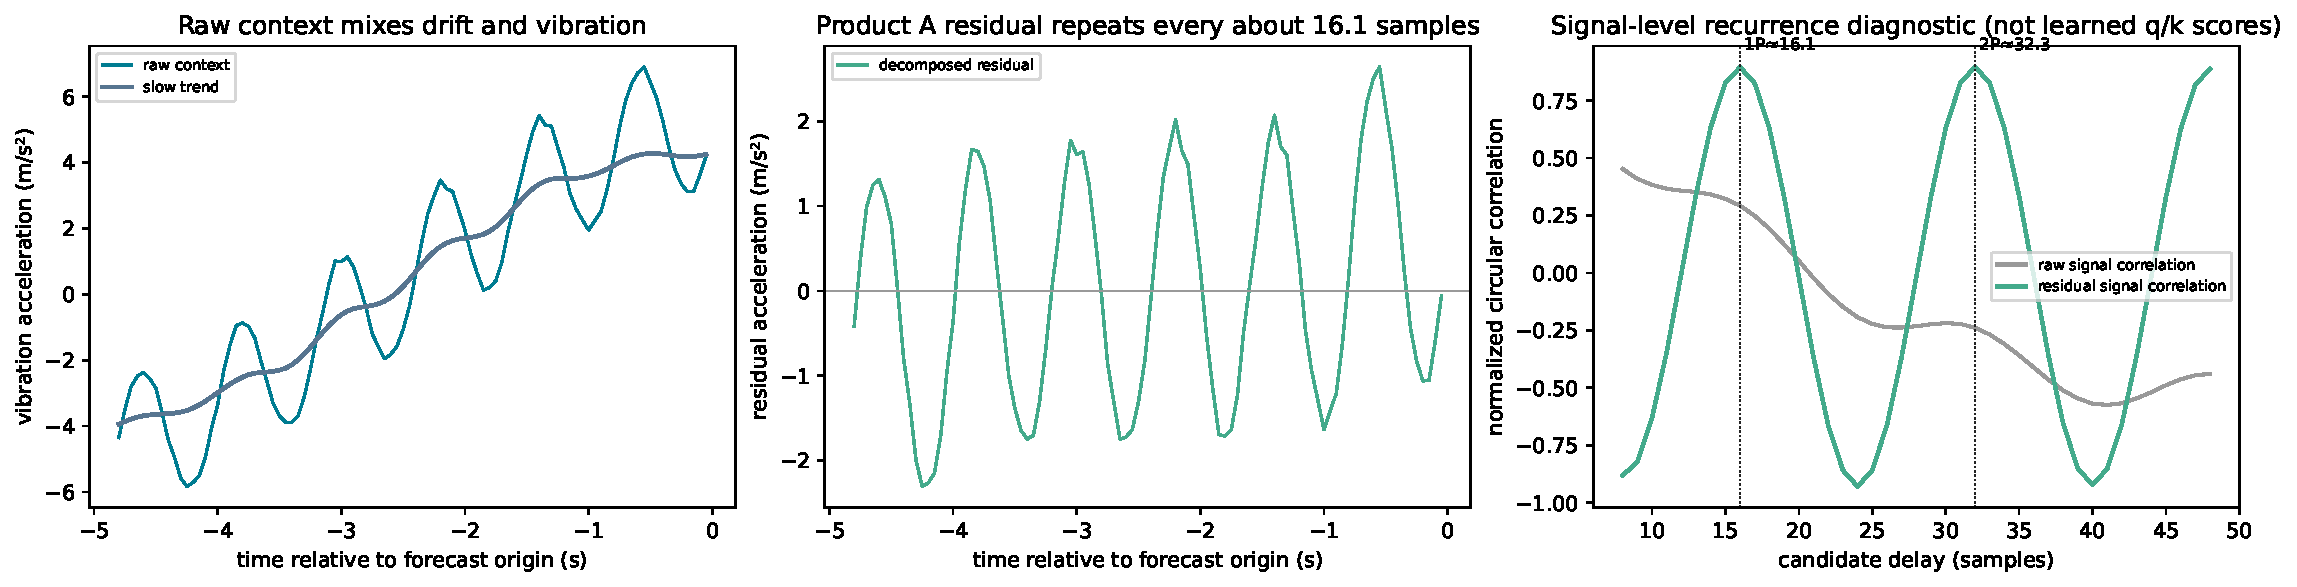
\includegraphics[width=\linewidth]{figures/t1_out3-2.pdf}
  \caption{Raw context and trend (left), remainder (middle) and circular correlation against delay for the raw signal and the remainder (right) of a Station 2 Product A validation context with $P = 16.1$ (Output 3.2).}
  \label{fig:t1-recurrence}
\end{figure}

\begin{table}[!htbp]
  \centering
  \caption{Residual correlation at the lags nearest $P$ and $2P$ for the window of Figure~\ref{fig:t1-recurrence} (Output 3.2).}
  \label{tab:t1-delays}
  \resizebox{\linewidth}{!}{\begin{tabular}{rlrrr}
\toprule
station & product & expected delay (samples) & nearest integer delay & residual signal correlation \\
\midrule
2 & Product A & 16.135 & 16 & 0.896 \\
2 & Product A & 32.269 & 32 & 0.897 \\
\bottomrule
\end{tabular}
}
\end{table}

\subsection{Comparing Designs and Deployment}
\label{subsec:t1-deploy}

\paragraph{Response 4(a).}

Decomposition should help most on contexts where the slow drift component is prominent. It addresses the slow drift directly by separating the trend part and sending it to a linear head, so the delay mixer sees the repeating part instead of a large steady rise.

\paragraph{Response 4(b).}

Each of the two switches, adding decomposition and replacing attention with delay mixing, helped alone on the established stations, cutting Raw Attention's RMSE from 0.424 to 0.296 with decomposition and to 0.219 with delay mixing, and both together reached 0.198 (RMSE and MSE for all models in Table~\ref{tab:t1-designs}). With the other switch already on, delay mixing lowered RMSE only from 0.296 to 0.198 and decomposition only from 0.219 to 0.198, so the gains overlapped rather than added up, likely because both switches deal with the same slow drift. Error grew with horizon for every model, as small phase errors build up over more steps, least for Autoformer-inspired (RMSE 0.133 at step 1 to 0.233 at step 48) and most for Raw Attention (0.145 to 0.533), and period routing was lowest at every step shown (Table~\ref{tab:t1-horizon}).

\paragraph{Response 4(c).}

We chose period-routed ridge for both populations before Output 4.3 ran. It had the lowest validation RMSE (0.166 on the established stations and 0.173 on Station 4), $6\times$ fewer parameters than any neural model and a 0.008\,s fit (Table~\ref{tab:t1-designs}). Its validation RMSE rose the least from the established stations to Station 4 (0.166 to 0.173, Table~\ref{tab:t1-designs}), as it never uses the station's identity.

\begin{table}[!htbp]
  \centering
  \caption{Validation RMSE (m/s$^2$) and MSE ((m/s$^2$)$^2$) of all fitted models, with trainable parameters and fitting time in seconds (cell 32 summary).}
  \label{tab:t1-designs}
  \resizebox{0.85\linewidth}{!}{\begin{tabular}{l cc cc rr}
\toprule
& \multicolumn{2}{c}{\textbf{Established (1--3)}} & \multicolumn{2}{c}{\textbf{Station 4}} & & \\
\cmidrule(lr){2-3}\cmidrule(lr){4-5}
\textbf{Model} & RMSE & MSE & RMSE & MSE & Params & Fit (s) \\
\midrule
Shared ridge & $0.767$ & $0.588$ & $0.876$ & $0.767$ & $4{,}608$ & $0.022$ \\
Sensor-specific ridge & $0.768$ & $0.590$ & -- & -- & $13{,}824$ & $0.003$ \\
Period-routed ridge & $0.166$ & $0.028$ & $0.173$ & $0.030$ & $59{,}904$ & $0.008$ \\
\midrule
Raw Attention & $0.424$ & $0.180$ & $0.617$ & $0.380$ & $368{,}368$ & $889.9$ \\
Attention + decomposition & $0.296$ & $0.088$ & $0.444$ & $0.197$ & $373{,}024$ & $1177.5$ \\
Raw delay mixer & $0.219$ & $0.048$ & $0.337$ & $0.114$ & $368{,}370$ & $882.7$ \\
Autoformer-inspired & $0.198$ & $0.039$ & $0.239$ & $0.057$ & $373{,}026$ & $1435.6$ \\
\bottomrule
\end{tabular}
}
\end{table}

\begin{table}[!htbp]
  \centering
  \caption{Validation RMSE (m/s$^2$) at forecast steps $h = 1, 12, 24, 48$ (Output 4.2).}
  \label{tab:t1-horizon}
  \resizebox{0.95\linewidth}{!}{\begin{tabular}{l cccc cccc}
\toprule
& \multicolumn{4}{c}{\textbf{Established (1--3)}} & \multicolumn{4}{c}{\textbf{Station 4}} \\
\cmidrule(lr){2-5}\cmidrule(lr){6-9}
\textbf{Model} & $h=1$ & $h=12$ & $h=24$ & $h=48$ & $h=1$ & $h=12$ & $h=24$ & $h=48$ \\
\midrule
Period-routed ridge & $0.112$ & $0.125$ & $0.147$ & $0.228$ & $0.119$ & $0.111$ & $0.153$ & $0.212$ \\
Raw Attention & $0.145$ & $0.331$ & $0.432$ & $0.533$ & $0.169$ & $0.478$ & $0.670$ & $0.775$ \\
Raw delay mixer & $0.120$ & $0.173$ & $0.186$ & $0.339$ & $0.137$ & $0.236$ & $0.273$ & $0.621$ \\
Attention + decomposition & $0.149$ & $0.228$ & $0.276$ & $0.399$ & $0.153$ & $0.344$ & $0.399$ & $0.592$ \\
Autoformer-inspired & $0.133$ & $0.162$ & $0.179$ & $0.233$ & $0.142$ & $0.185$ & $0.237$ & $0.297$ \\
\bottomrule
\end{tabular}
}
\end{table}

\FloatBarrier
\section{Long-Horizon Forecasting with Autoformer}
\label{sec:t2}

We forecast the next 168 values (\texttt{time\_idx} 43657 to 43824) of an anonymised, non-negative and heavy-tailed series from its first 43,656 values, with ten optional covariates given for every step including the horizon. The model is an Autoformer \citep{wu2021autoformer}, which repeats moving-average decomposition in every layer and mixes values at the top-$k$ time delays found by autocorrelation instead of point-wise attention \citep{vaswani2017attention}. The Autoformer's series decomposition handles the series' slow drift and its delay mixing exploits the 24-step periodicity, making it a natural fit for this long-horizon task.

\subsection{Data and Validation}
\label{subsec:t2-data}

We z-scored the target and the six continuous covariates (A to F) on training rows only, so they enter the model on the same scale. The four one-hot indicators (G to J) are already unit-scaled and were kept as they are. Forecasts were clipped at 0 because the series is non-negative and the model can otherwise predict negative values. The index has no dates, so we estimated the period from the training data. The detrended periodogram peaked at 24.0 steps (Figure~\ref{fig:t2-acf}), so we set the moving-average kernel to 25 (one period plus one, as an odd width lets the centred average line up exactly with each time step). The autocorrelation of the training series fell to 0.033 by lag 168 (Table~\ref{tab:t2-period}), so values 168 steps apart are almost uncorrelated.

We validated on the last $12 \times 168$ steps (\texttt{time\_idx} 41641 to 43656), using the mean per-origin RMSE, MAE and sMAPE over 78 origins spaced 24 steps apart. Many origins give a less noisy estimate than one block, and spacing them one period apart starts every forecast at the same phase of the 24-step cycle. A single 168-step block is still noisy, as the naive forecast (mean of the last 168 values) had an RMSE of 120.56 with a block sd of 29.01 (Table~\ref{tab:t2-exog}). Every comparison therefore used 3 seeds, and two settings counted as different only if their mean RMSE differed by more than twice the standard error.

\begin{figure}[!htbp]
  \centering
  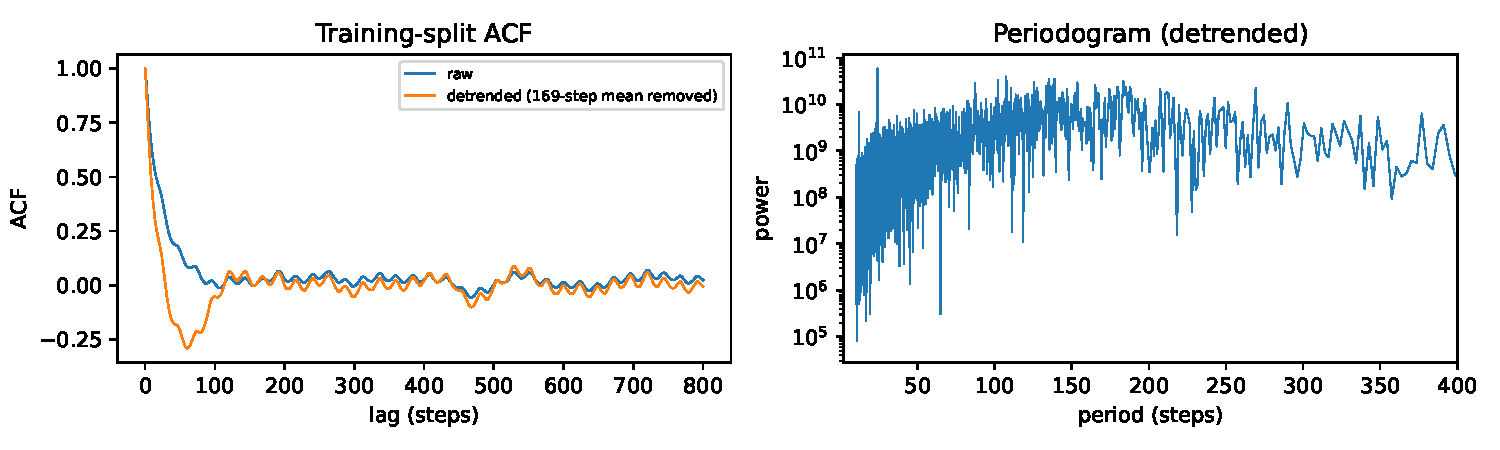
\includegraphics[width=\linewidth]{figures/t2_acf.pdf}
  \caption{Autocorrelation of the raw and detrended training split (left) and periodogram of the detrended series (right), \texttt{time\_idx} 1 to 41640.}
  \label{fig:t2-acf}
\end{figure}

\begin{table}[!htbp]
  \centering
  \caption{Autocorrelation of the training split and its largest periodogram peak. Detrending removes a centred 169-step moving average.}
  \label{tab:t2-period}
  \begin{tabular}{lccccc}
\toprule
\textbf{ACF at lag} & 1 & 12 & 24 & 48 & 168 \\
\midrule
Raw & $0.965$ & $0.566$ & $0.404$ & $0.174$ & $0.033$ \\
Detrended & $0.948$ & $0.364$ & $0.129$ & $-0.192$ & $0.040$ \\
\midrule
\multicolumn{6}{l}{Largest periodogram peak (detrended) at a period of 24.0 steps} \\
\bottomrule
\end{tabular}

\end{table}

\subsection{Model}
\label{subsec:t2-model}

Our encoder-decoder Autoformer reuses the decomposition and delay functions of Section~\ref{sec:t1}, with the layer order and decoder initialisation of the official implementation \citep{thuml2021autoformercode}. Every layer re-decomposes its hidden values, all mixing is Auto-Correlation over $k = \lfloor c \ln L \rfloor$ delays, and over the forecast steps the decoder's seasonal input starts at zero and its trend input at the mean of the input window (Table~\ref{tab:t2-settings}), so the model never sees the true future values and must build the forecast from the encoder output and the selected delays.

Changing one setting at a time (Table~\ref{tab:t2-arms}), only an input length of 720 beat the base (RMSE 78.50 $\pm$ 1.16 against 81.48 $\pm$ 1.62), likely because a longer window holds more repeats of the 24-step cycle. A log1p target had the lowest MAE (60.80) and sMAPE (58.70) but a higher RMSE (88.82) and a bias of $-24.64$, because minimising squared error on log-transformed values pulls predictions toward the geometric mean, which is always lower than the true mean, so high peaks are underestimated. We kept the raw target, since ranking uses RMSE. Validation RMSE was best after $E^{*} = 2$ epochs, because the learning rate halves every epoch, so later epochs barely change the weights.

\begin{table}[!htbp]
  \centering
  \caption{Validation results when one setting of the future-covariate model is changed, mean $\pm$ sd over 3 seeds. Block sd is the sd of RMSE across the 12 non-overlapping 168-step blocks.}
  \label{tab:t2-arms}
  \resizebox{\linewidth}{!}{\begin{tabular}{l c c c c c r}
\toprule
\textbf{Model} & RMSE & MAE & sMAPE (\%) & Bias & Block sd & $\mathcal{P}$ \\
\midrule
Base (future covariates) & $81.48$ $\pm$ $1.62$ & $63.50$ & $74.09$ & $2.94$ & $17.90$ & $30{,}593$ \\
$L = 168$ & $82.90$ $\pm$ $0.64$ & $63.40$ & $80.85$ & $-5.37$ & $21.04$ & $30{,}593$ \\
$L = 720$ & $78.50$ $\pm$ $1.16$ & $60.05$ & $75.79$ & $-2.46$ & $15.33$ & $30{,}593$ \\
Kernel 49 & $82.38$ $\pm$ $1.04$ & $62.60$ & $74.70$ & $-1.68$ & $18.62$ & $30{,}593$ \\
$d = 64$ & $86.89$ $\pm$ $4.60$ & $68.04$ & $78.17$ & $4.10$ & $21.22$ & $93{,}953$ \\
Learning rate $10^{-3}$ & $84.48$ $\pm$ $4.00$ & $67.47$ & $84.13$ & $9.12$ & $20.09$ & $30{,}593$ \\
log1p target & $88.82$ $\pm$ $0.62$ & $60.80$ & $58.70$ & $-24.64$ & $28.14$ & $30{,}593$ \\
\bottomrule
\end{tabular}
}
\end{table}

\begin{table}[!htbp]
  \centering
  \caption{Settings of the final model.}
  \label{tab:t2-settings}
  \small
  \begin{tabular}{ll}
\toprule
\textbf{Setting} & \textbf{Value} \\
\midrule
Covariates & future \\
Input length $L$ & 720 \\
Label length & 168 \\
Moving-average kernel & 25 \\
Factor $c$ & 1 \\
$d_{\text{model}}$, heads, $d_{\text{ff}}$ & 32, 4, 64 \\
Encoder, decoder layers & 2, 1 \\
Dropout & 0.1 \\
Optimiser & Adam, lr $0.0001$ halved each epoch, batch 32 \\
Epochs per member $E^{*}$ & 2 \\
Ensemble seeds & 0, 1, 2, 3, 4 \\
\bottomrule
\end{tabular}

\end{table}

\subsection{External Data}
\label{subsec:t2-exog}

Only the covariates over the forecast horizon helped (Table~\ref{tab:t2-exog}). Fed to the decoder, which covers the label and forecast steps, they lowered RMSE from 117.31 $\pm$ 0.33 to 81.48 $\pm$ 1.62, while past covariates in the encoder (which looks at history) tied (117.20 $\pm$ 0.37) and both together did worse (89.92 $\pm$ 8.28). The future covariates describe future conditions that cannot be inferred from the target's history alone, and without them the model barely beat the naive forecast (120.56). Past covariate values likely added little because the encoder already sees the target's own past. The worse result when both were used suggests that adding uninformative encoder inputs introduced noise that interfered with learning from the useful future covariates.

\begin{table}[!htbp]
  \centering
  \caption{Validation results with and without the optional file ($L = 336$), mean $\pm$ sd over 3 seeds. Past covariates enter the encoder, future covariates the decoder over the label and forecast steps.}
  \label{tab:t2-exog}
  \resizebox{\linewidth}{!}{\begin{tabular}{l c c c c c r}
\toprule
\textbf{Model} & RMSE & MAE & sMAPE (\%) & Bias & Block sd & $\mathcal{P}$ \\
\midrule
Naive (last-168 mean) & $120.56$ & $99.15$ & $94.96$ & $-0.37$ & $29.01$ & -- \\
\midrule
No covariates & $117.31$ $\pm$ $0.33$ & $97.33$ & $95.21$ & $-1.34$ & $26.62$ & $29{,}633$ \\
Past covariates & $117.20$ $\pm$ $0.37$ & $97.33$ & $94.89$ & $-1.00$ & $27.31$ & $30{,}593$ \\
Future covariates & $81.48$ $\pm$ $1.62$ & $63.50$ & $74.09$ & $2.94$ & $17.90$ & $30{,}593$ \\
Past and future & $89.92$ $\pm$ $8.28$ & $71.79$ & $79.48$ & $9.36$ & $22.52$ & $31{,}553$ \\
\bottomrule
\end{tabular}
}
\end{table}

\subsection{Final Model and Leaderboard}
\label{subsec:t2-final}

Over five seeds the chosen model averaged 81.18 $\pm$ 3.24, so the improvement seen with $L = 720$ over 3 seeds was partly noise, and averaging the five forecasts lowered RMSE to 79.75 (Table~\ref{tab:t2-final}). Each seed was retrained for 2 epochs on all 43,656 observations, giving $\mathcal P = 152{,}965$ trainable parameters and $\mathcal E = 10$ epochs, summed over the five models. The leaderboard RMSE of 84.81 is within one block sd (16.65) of validation.

\begin{table}[!htbp]
  \centering
  \caption{Validation results of the final configuration per seed and for the five-seed ensemble. The ensemble's $\mathcal P$ and $\mathcal E$ are summed over the five members retrained on all observations.}
  \label{tab:t2-final}
  \small
  \begin{tabular}{l c c c c r r}
\toprule
\textbf{Model} & RMSE & MAE & sMAPE (\%) & Block sd & $\mathcal{P}$ & $\mathcal{E}$ \\
\midrule
Seed 0 & $79.70$ & & & & $30{,}593$ & 2 \\
Seed 1 & $79.33$ & & & & $30{,}593$ & 2 \\
Seed 2 & $77.63$ & & & & $30{,}593$ & 2 \\
Seed 3 & $84.65$ & & & & $30{,}593$ & 2 \\
Seed 4 & $84.58$ & & & & $30{,}593$ & 2 \\
Seeds 0--4, mean $\pm$ sd & $81.18$ $\pm$ $3.24$ & $62.21$ & $74.89$ & $17.08$ & & \\
\midrule
Ensemble of seeds 0--4 & $79.75$ & $60.78$ & $69.60$ & $16.65$ & $152{,}965$ & 10 \\
\bottomrule
\end{tabular}

\end{table}

\bibliographystyle{plainnat}
\bibliography{ref}

\appendix

\section{Generative AI Disclosure}
\label{app:ai}

Claude Code was used for code scaffolding, and debugging Task 2 code and experiments, as well as structural draft and minor style-edit suggestions for the report prose. It was used with the VibeWise plugin (\url{https://github.com/nykooi1/vibe-wise}), which has Claude ask for our approach first, discuss tradeoffs and explain unfamiliar concepts before writing a single line of code.

\end{document}
